\documentclass[UTF8]{ctexart}

\usepackage{graphicx}
\usepackage{float}
\usepackage{amsmath,amssymb,amsfonts}

\begin{document}
	
	\section*{Ans\_2}
	问题二对应的程序如下:
	
	
	\sffamily
	\% 定义圆环的内外半径
	
	R = 3; \% 外半径
	
	r = 1; \% 内半径(环的宽度由这个参数和后续计算中的cos(θ)决定)
	
	\vspace*{1\baselineskip}
	\% 生成参数$\theta$和$\phi$的网格
	
	\vspace*{1\baselineskip}
	[theta, phi] = meshgrid(linspace(0, 2*pi, 50), linspace(0, 2*pi, 50));
	
	\vspace*{1\baselineskip}
	\% 计算x, y, z坐标
	
	x = (R + r * cos(theta)) .* cos(phi);
	
	y = (R + r * cos(theta)) .* sin(phi);
	
	z = r * sin(theta);
	
	\vspace*{1\baselineskip}
	\% 使用surf函数绘制三维图像
	
	figure;
	
	surf(x, y, z);
	
	\vspace*{1\baselineskip}
	\% 添加图形标签和标题
	
	xlabel('X');
	
	ylabel('Y');
	
	zlabel('Z');
	
	title('圆环函数');
	
	\vspace*{1\baselineskip}
	\% 设置图形视角
	
	view(3); \% 或者使用其他视角
	
	\vspace*{1\baselineskip}
	\% 添加光照效果(可选)
	
	shading interp; \% 平滑着色
	
	colormap jet;   \% 设置颜色映射
	
	colorbar;      \% 显示颜色条
	
	lighting gouraud; \% Gouraud光照
	
	\vspace*{1\baselineskip}
	\% 如果需要,可以添加网格线
	
	grid on;
	
	\vspace*{1\baselineskip}
	\rmfamily
	该程序首先定义了圆环的内外半径$R$和$r$,然后生成了一个$\theta$和$\phi$的网格,这些网格点覆盖了整个圆环面。接下来,程序计算了每个网格点上的$x,y,z$坐标,并使用surf函数绘制了三维图像。最后,程序添加了图形标签、标题、光照效果和网格线。
	
	\centerline{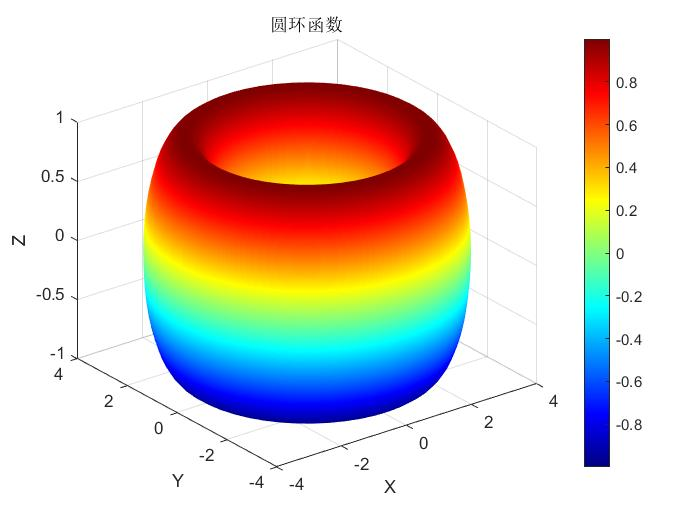
\includegraphics[width=0.7\textwidth]{figure_for_ans_2}}
	
	
\end{document}
